\begin{abcliste}
\abc Die Steigung des $v(t)$-Graphen ist die Beschleunigung $-g$. In der Zeit $t_\mathrm{L}$ ändert sich die Geschwindigkeit um $-2v_0$:
\begin{align}
 -g &= \frac{-v_0-v_0}{t_\mathrm{L}} \quad\Rightarrow\quad t_\mathrm{L} = \tLF = \frac{2\cdot\vNull}{\ncg} = \tL \approx \result{\tLP{0}{2}}
\end{align}

\abc Die Ortsänderung ist die Fläche unter dem $v(t)$-Graphen mit Vorzeichen. Der Graph schneidet die $t$-Achse genau in der Mitte, bei $t_\mathrm{L}/2$ (dort ist der Ball am höchsten Punkt). Die beiden Dreiecke über und unter der Achse sind gleich gross:
\begin{center}
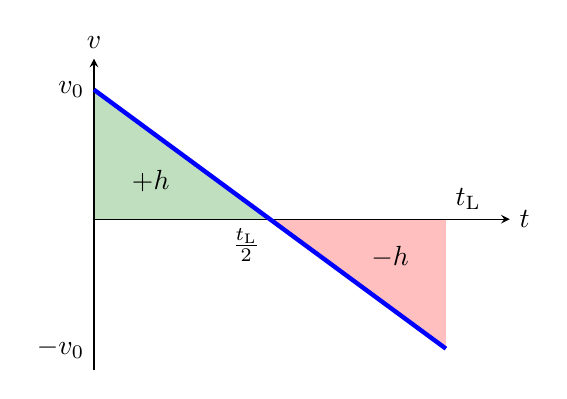
\begin{tikzpicture}[>=stealth, x=1.6cm, y=0.12cm]
 \fill[green!50!black, opacity=0.25] (0,0) -- (0,13.7) -- (1.3965,0) -- cycle;
 \fill[red, opacity=0.25] (1.3965,0) -- (2.793,-13.7) -- (2.793,0) -- cycle;
 \draw[->] (0,0) -- (3.3,0) node[right] {$t$};
 \draw[->] (0,-16) -- (0,17) node[above] {$v$};
 \draw[ultra thick, blue] (0,13.7) -- (2.793,-13.7);
 \node[left] at (0,13.7) {$v_0$};
 \node[left] at (0,-13.7) {$-v_0$};
 \node[below left] at (1.3965,0) {$\frac{t_\mathrm{L}}{2}$};
 \node[above right] at (2.793,0) {$t_\mathrm{L}$};
 \node at (0.45,4) {$+h$};
 \node at (2.35,-4) {$-h$};
\end{tikzpicture}
\end{center}
Ihre Flächen heben sich auf: $\Delta s = h - h = 0$. Der Ball ist $\result{\text{wieder am Abwurfort}}$ (er wird ja auf derselben Höhe aufgefangen).

\abc Für die zurückgelegte Strecke zählen beide Dreiecke positiv. Ein Dreieck entspricht der Steighöhe
\begin{align}
 h &= \hMaxF = \frac{1}{2}\cdot\vNull\cdot\frac{\tL}{2} = \hMax
\end{align}
und die Strecke ist
\begin{align}
 d &= \distF = 2\cdot\hMax = \dist \approx \result{\distP{0}{2}}
\end{align}
\end{abcliste}
